\section*{Direction 2. Prey growth and predator competition}
\subsection*{Abstract}
We crossed three prey growth laws with two levels of direct predator competition while keeping the feeding law fixed. Logistic growth gives one globally attracting coexistence state whenever predators can invade. Weak and strong Allee growth each allow three coexistence states. Strong Allee growth also creates an extinction basin at low prey density. A matched-equilibrium comparison establishes how the growth law orders predator abundance as competition increases. Four held-out algae--rotifer experiments distinguish these mathematical effects from predictive gains. All six models improved on persistence for one-step prediction, but a constant training mean gave the lowest average free-running error.

\subsection*{Results}
Let $x$ denote prey density, $y$ predator density, and $P=mxy/(\beta+y)$ their common feeding rate. The six systems have the form
\[
 \dot x=xg(x)-P,\qquad \dot y=eP-dy-hy^2.
\]
The course model is M0. Its denominator $\beta+y$ already reduces intake per predator as predator density rises. Direct competition adds the loss $hy^2$. Here $m,\beta,e,d,r,K>0$, $\alpha>0$, and $0<A<K$. Under weak Allee growth, per-capita growth rises near zero when $\alpha K>1$. Under strong Allee growth it is negative for $0<x<A$.

\begin{center}
\begin{tabular}{@{}llcc@{}}\toprule
Prey growth & Per-capita rate $g(x)$ & $h=0$ & $h>0$\\\midrule
Logistic (L) & $r(1-x/K)$ & M1 & M3\\
Weak Allee (W) & $r(1-x/K)(1+\alpha x)$ & M0 & M4\\
Strong Allee (S) & $r(1-x/K)(x/A-1)$ & M2 & M5\\\bottomrule
\end{tabular}
\end{center}

\textbf{Survival and stability.} All six systems preserve positive populations and keep them bounded. The per-capita growth rate of a rare predator at $(K,0)$ is $\lambda_K=emK/\beta-d$. When $\lambda_K\leq0$, every strictly positive trajectory with logistic or weak Allee growth tends to $(K,0)$. When $\lambda_K>0$, both populations eventually stay above positive lower bounds under either law. Logistic growth then gives global attraction to one interior equilibrium. Weak Allee growth permits multiple equilibria. A positive equilibrium with prey density $x_*\ge K-1/\alpha$ attracts every strictly positive trajectory. With strong growth, any start with $0<x\leq A$ and $y>0$ leads to extinction. The full basin boundaries remain open in some cases with coexistence.

\textbf{Enrichment and bifurcations.} At fixed growth-shape parameters, increasing $K$ raises both equilibrium densities on a hyperbolically stable interior branch. All six systems have a transcritical exchange at $\lambda_K=0$. Each of the four Allee models has separate admissible examples of a saddle-node, a Hopf bifurcation, and a Bogdanov--Takens point. A Hopf crossing can therefore change stability even while the equilibrium densities increase.

\begin{center}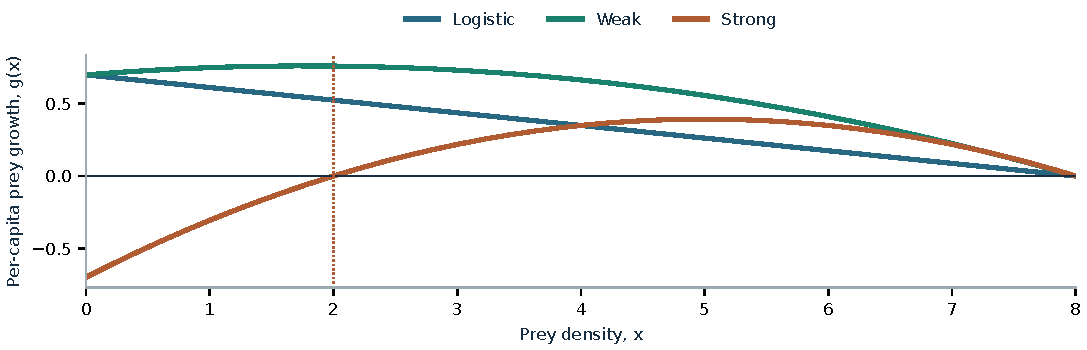
\includegraphics[width=.72\linewidth]{d2/repro/figures/growth.pdf}\end{center}
{\small\textbf{Figure 2.1.} Per-capita prey growth for $r=0.7$, $K=8$, $\alpha=0.225$, and $A=2$. Only strong Allee growth is negative below the threshold $A$.\par}

\clearpage
\subsection*{Equilibria, trajectories, and population removal}
At coexistence set $z=y/\beta$, $s=\beta d/(em)$, and $\kappa=h\beta/d$. The predator equation gives $x=s(1+z)(1+\kappa z)$. Substitution in the prey equation gives
\[
 H(z)=(1+z)g\!\left(s(1+z)(1+\kappa z)\right)-mz=0 .
\]
Each positive root gives one coexistence state. Logistic growth allows at most one. For each Allee law the upper bound is three, counting multiplicity, with rational examples attaining three distinct roots in both competition arms. For example, take $g(x)=1/5+27x/200-x^2/50$, $s=33/76$, and $m=399/800$. For both $\kappa=0$ and $\kappa=32/45045$, the signs of $H$ at $3,7/2,9/2,6$ are $+,-,+,-$. Continuity gives three distinct positive roots in each case. The table uses a separate shared baseline.

\begin{center}\small
\begin{tabular}{@{}llcc@{}}\toprule
Law & Model & Attracting $(x,y)$ & Saddle $(x,y)$\\\midrule
Logistic & M1 & $(5.526,3.110)$ & ---\\
Logistic with competition & M3 & $(5.842,2.038)$ & ---\\
Weak Allee & M0 & $(6.959,4.228)$ & ---\\
Weak Allee with competition & M4 & $(7.109,2.498)$ & ---\\
Strong Allee & M2 & $(6.915,4.194)$ & $(2.466,0.724)$\\
Strong Allee with competition & M5 & $(7.091,2.491)$ & $(2.340,0.469)$\\\bottomrule
\end{tabular}
\end{center}

\begin{center}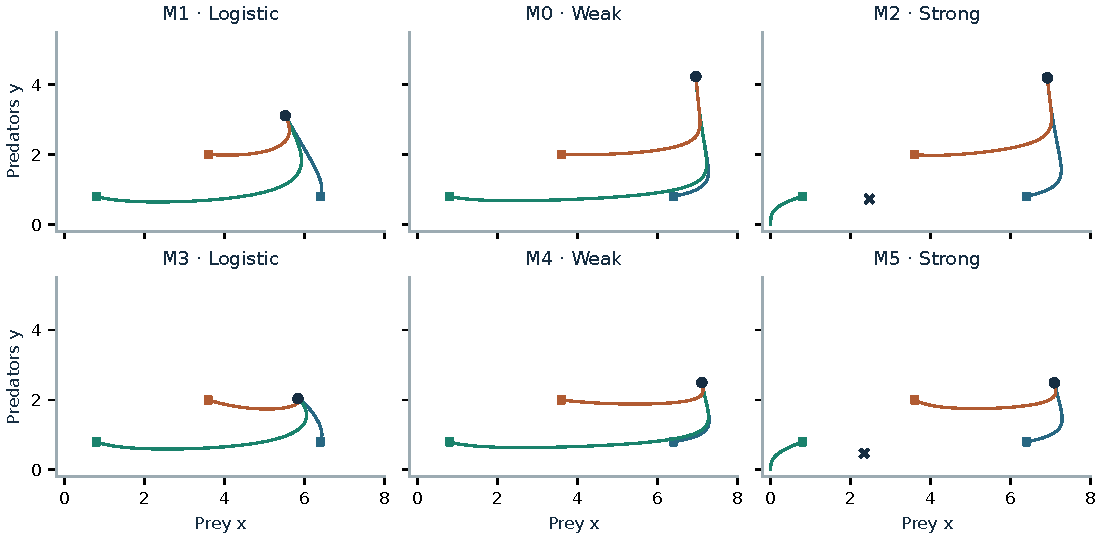
\includegraphics[width=.97\linewidth]{d2/repro/figures/phase.pdf}\end{center}
{\small\textbf{Figure 2.2.} Six models, three common starting states. Squares mark $(6.4,0.8)$, $(0.8,0.8)$, and $(3.6,2)$. Circles mark attracting coexistence states and crosses mark saddles. The table and figure use $r=0.7$, $K=8$, $\alpha=0.225$, $A=2$, $m=0.3$, $\beta=1.2$, $e=0.65$, and $d=0.25$. The lower row uses $h=0.05$.\par}

\textbf{Shocks.} From each model's high-prey attracting equilibrium we removed 5, 25, 60, or 85\% of either species. In 45 of 48 runs both populations recovered to within 2\% of their starting densities and stayed there for at least the last 50 time units of a 600-unit run. After 60\% prey removal, both strong-growth models still started above $A=2$. M2 went extinct from $x=2.766$, while M5 recovered from $x=2.836$ in 17.5 time units. The predator density present after removal helps determine which side of the recovery boundary the system reaches.

\clearpage
\subsection*{Matched competition and held-out prediction}
For the mathematical comparison, we calibrated one growth-rate coefficient per law so that the three models shared $(x_0,y_0)$ at $h=0$. At each later $h$ while the three equilibrium branches remain positive with positive determinant, the strong law has the most predators and the logistic law has the fewest. This comparison concerns the branch connected to the matched starting point. Figure~2.3 also shows how the common interval can end. The choice of matching matters in the wider simulation study. Across 24 matched runs, the weak-minus-logistic contrast in the competition effect on mean late predator density was $-1.401$ at equal $r$ and $+0.355$ when growth rates were matched at $0.6K$.

\begin{center}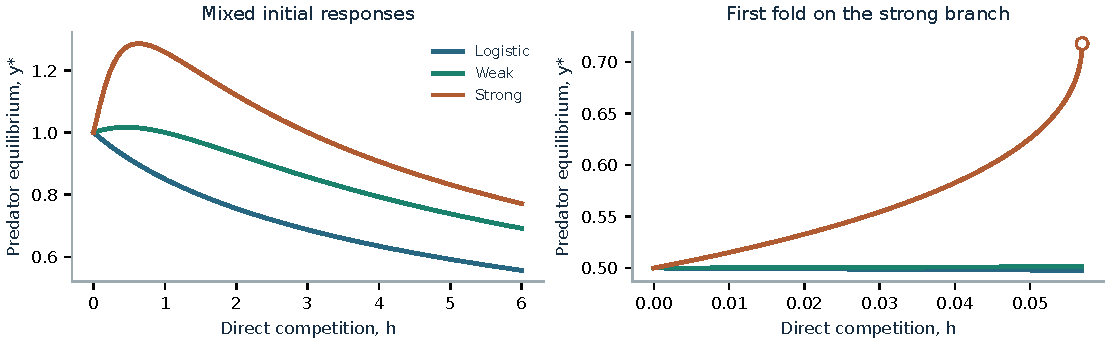
\includegraphics[width=.98\linewidth]{d2/repro/figures/ordering.pdf}\end{center}
{\small\textbf{Figure 2.3.} Predator abundance against competition strength. Left, the common start is $(4,1)$, and at $h=6$ predator densities are $0.5564$ (L), $0.6915$ (W), and $0.7711$ (S). Right, the strong branch reaches a fold at $h\simeq0.056907$ in a separate example with $K=4$.\par}

\textbf{Empirical comparison.} Each fold fitted three chemostat experiments and predicted the fourth. A one-step forecast starts from the previous observation. A free-running forecast starts only once. Scores are the mean of the two species' root mean square errors, each divided by its training standard deviation or by $0.1$ if that deviation is smaller, then averaged equally across four held-out experiments. Lower scores indicate smaller errors.

\begin{center}\small
\begin{tabular}{@{}lrr@{}}\toprule
Model or reference & One-step error & Free-running error\\\midrule
M0 weak & 0.8858 & 1.0420\\
M1 logistic & 0.8849 & 1.0376\\
M2 strong & 0.8990 & 1.0802\\
M3 logistic with competition & \textbf{0.8825} & 1.0582\\
M4 weak with competition & 0.8855 & 1.0621\\
M5 strong with competition & 0.8966 & 1.0978\\
Persistence & 1.0403 & 2.1521\\
Training mean & 1.0370 & \textbf{1.0370}\\
Training drift & 1.0403 & 2.3607\\\bottomrule
\end{tabular}
\end{center}
M3 reduced mean one-step error by 15.2\% relative to persistence and by 0.270\% relative to M1. In all 48 free-running records, the 95th minus the 5th percentile in the final half of the time span was below 5\% of the corresponding training standard deviation. Observed prey minima also exceeded every fitted strong Allee threshold. The records therefore provide no direct observation of a threshold crossing. Data and study design come from Blasius et al., \emph{Nature} 577 (2020), 226--230 \href{https://doi.org/10.1038/s41586-019-1857-0}{(article)} and the \href{https://doi.org/10.6084/m9.figshare.10045976.v1}{public observations}.

\clearpage
\subsection*{Mathematical proof of the matched competition order}
\textbf{Statement.} Fix $K,m,\beta,e,d>0$, choose $0<A<x_0<K$, $\alpha K>1$, $\alpha>0$, and choose $y_0>0$ satisfying $emx_0=d(\beta+y_0)$. Write $q=my_0/(\beta+y_0)$ and $U(x)=(K-x)/(K-x_0)$. Calibrate the three growth rates to
\[
 g_L=qU,\qquad g_W=qU\frac{1+\alpha x}{1+\alpha x_0},\qquad
 g_S=qU\frac{x-A}{x_0-A} .
\]
Assume each initial equilibrium has positive Jacobian determinant. Its local equilibrium branch exists by the implicit function theorem. On any common connected interval starting at zero on which the three branches have positive coordinates and positive determinants, every $h>0$ satisfies
\[
 y_S(h)>y_W(h)>y_L(h),\qquad x_S(h)>x_W(h)>x_L(h)>x_0 .
\]
The right derivatives at zero also satisfy $y_S'(0)>y_W'(0)>y_L'(0)$. Adding negative trace restricts the statement to attracting equilibria.

\textit{Proof.} At a positive equilibrium let $J=\left(\begin{smallmatrix}a&b\\c&-D\end{smallmatrix}\right)$, where
\[
 a=xg'(x),\quad b=-\frac{mx\beta}{(\beta+y)^2},\quad
 c=\frac{emy}{\beta+y},\quad D=y\left(\frac{emx}{(\beta+y)^2}+h\right).
\]
Set $B=-bc>0$ and $\Delta=B-Da$. Differentiating the two zero equations with respect to $h$ gives $J(x',y')^{\mathsf T}=(0,y^2)^{\mathsf T}$. Therefore
\[
 x'=-\frac{by^2}{\Delta}>0,\qquad y'=\frac{ay^2}{\Delta} .
\]
At the common start the three logarithmic growth slopes share the term $-1/(K-x_0)$. The remaining terms are $0$, $\alpha/(1+\alpha x_0)$, and $1/(x_0-A)$, in increasing order, since their last difference is $(1+\alpha A)/[(x_0-A)(1+\alpha x_0)]>0$. The three growth rates agree there, so $a_S>a_W>a_L$. The other Jacobian entries are shared at the start. Subtraction gives
\[
 y_i'(0)-y_j'(0)=\frac{y_0^2B(a_i-a_j)}{\Delta_i\Delta_j}.
\]
This orders the initial derivatives and therefore the predator densities for small $h>0$.

Each branch moves to $x>x_0$, and $g_i(x)=my/(\beta+y)>0$ forces $x<K$. On $(x_0,K)$ the multipliers of $qU(x)$ are $1$, $1+\alpha(x-x_0)/(1+\alpha x_0)$, and $1+(x-x_0)/(x_0-A)$. Hence $g_S>g_W>g_L$ there. A later equality of two predator densities at the same $h$ would force a common prey density through $x=(\beta+y)(d+hy)/(em)$, then equal growth rates through the prey equations. This contradicts the strict growth order. Continuity proves the predator ranking throughout. The same expression for $x$ is strictly increasing in $y$ at fixed $h$, proving the prey ranking.\hfill$\square$

\textbf{An exact example.} For $K=10$, $x_0=4$, $y_0=A=\alpha=m=\beta=1$, $e=2$, and $d=4$, the calibrated growth coefficients are $r_L=5/6$, $r_W=1/6$, and $r_S=5/18$. Substitution gives $y_L'(0)=-1/5$, $y_W'(0)=1/13$, and $y_S'(0)=1$. Competition initially lowers predator density with logistic growth and raises it with either Allee law. The finite theorem ranks the densities even where a branch later changes direction, as in the left panel of Figure~2.3.

\clearpage
\subsection*{Python code and numerical checks}
This Python example uses the matched equilibrium $(4,1)$ on the preceding page. For each growth law it calculates $a=x_0g'(x_0)$, the determinant $\Delta=B-Da$, and the initial predator response $y'(0)=ay_0^2/\Delta$.

\begin{lstlisting}[language=Python,basicstyle=\ttfamily\footnotesize]
from fractions import Fraction as F

x0, y0, K, A, alpha = 4, 1, 10, 1, 1
m, beta, e = 1, 1, 2
q = F(m*y0, beta + y0)
b = -F(m*x0*beta, (beta + y0)**2)
c = F(e*m*y0, beta + y0)
D = F(y0*e*m*x0, (beta + y0)**2)  # h = 0
for extra in (0, F(alpha, 1 + alpha*x0), F(1, x0 - A)):
    a = x0*q*(-F(1, K - x0) + extra)
    determinant = -b*c - D*a
    assert determinant > 0
    print(a*y0**2 / determinant)
\end{lstlisting}
The output, in logistic, weak Allee, and strong Allee order, is $-1/5$, $1/13$, and $1$. The larger numerical check isolated the positive roots of 29 rational examples, checked 12 bifurcation cases, confirmed recovery in 45 of 48 disturbance runs, and recalculated the held-out forecast errors. Across 18 reintegrated trajectories, the largest difference divided by one plus the magnitude of the original coordinate was $2.5\times10^{-8}$.

\subsection*{Lean verification results}
Lean 4.19.0 with Mathlib v4.19.0 checked 47 public declarations. It verified local branch existence from a common equilibrium and the strict order of the initial predator derivatives. It also proved the ordering of both populations on any connected branch segment from that equilibrium where all coordinates and determinants stay positive. For each Allee law, Lean verified the bound of three positive roots, counting multiplicity, and exact examples attaining it with zero and with positive competition. The recovery rates, trajectories, and forecast scores were checked numerically.
